\documentclass[tikz,border=10pt]{standalone}
\usepackage{tikz}
\usetikzlibrary{calc}
\begin{document}
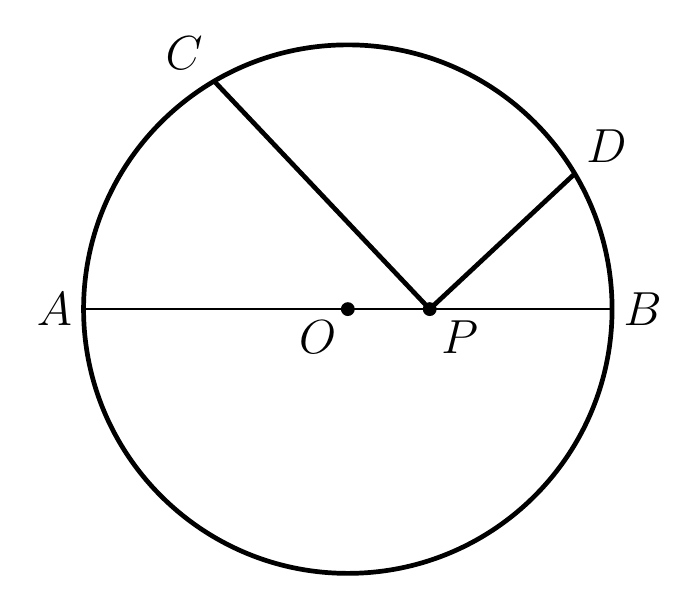
\begin{tikzpicture}[line width=1.7pt, line join=round]
  % Coordinates in cm (s = 0.021333 cm/px, origin at O)
  \coordinate (O) at (0,0);
  \coordinate (A) at (-3.356,0);     % left end of diameter
  \coordinate (B) at (3.356,0);      % right end of diameter
  \coordinate (P) at (1.04,0);       % point on AB between O and B
  % C and D recomputed exactly on circle of radius 3.356 centred at O
  \coordinate (C) at (-1.6975,2.8951); % upper-left point on circle
  \coordinate (D) at (2.8824,1.7202);  % upper-right point on circle

  % Circle and diameter (diameter thinned to ~0.9pt)
  \draw (O) circle (3.356);
  \draw[line width=0.9pt] (A) -- (B);

  % Segments from P, ending exactly on the circle
  \draw (P) -- (C);
  \draw (P) -- (D);

  % Larger filled dots at O and P
  \fill (O) circle (2.5pt);
  \fill (P) circle (2.5pt);

  % Labels
  \node[left, font=\fontsize{17}{20.4}\selectfont] at (A) {$A$};
  \node[right, font=\fontsize{17}{20.4}\selectfont] at (B) {$B$};
  \node[below left, font=\fontsize{17}{20.4}\selectfont] at (O) {$O$};
  \node[below right, font=\fontsize{17}{20.4}\selectfont] at (P) {$P$};
  \node[above left, font=\fontsize{17}{20.4}\selectfont] at (C) {$C$};
  \node[above right, font=\fontsize{17}{20.4}\selectfont] at (D) {$D$};
\end{tikzpicture}
\end{document}